%%%%%%%%%%%%%%%%%%%%%%%%%%%%%%%%%%%%%%%%%
% Wilson Resume/CV
% XeLaTeX Template
% Version 1.0 (22/1/2015)
%
% This template has been downloaded from:
% http://www.LaTeXTemplates.com
%
% Original author:
% Howard Wilson (https://github.com/watsonbox/cv_template_2004) with
% extensive modifications by Vel (vel@latextemplates.com)
%
% License:
% CC BY-NC-SA 3.0 (http://creativecommons.org/licenses/by-nc-sa/3.0/)
%
%%%%%%%%%%%%%%%%%%%%%%%%%%%%%%%%%%%%%%%%%

%----------------------------------------------------------------------------------------
%	PACKAGES AND OTHER DOCUMENT CONFIGURATIONS
%----------------------------------------------------------------------------------------
\documentclass[11pt]{article} % Default font size
\usepackage{graphicx}
\graphicspath{ {images/} }
\thispagestyle{empty}
% * <spencer.tengz@gmail.com> 2018-04-27T13:12:11.200Z:
%
% ^.
%%%%%%%%%%%%%%%%%%%%%%%%%%%%%%%%%%%%%%%%%
% Wilson Resume/CV
% Structure Specification File
% Version 1.0 (22/1/2015)
%
% This file has been downloaded from:
% http://www.LaTeXTemplates.com
%
% License:
% CC BY-NC-SA 3.0 (http://creativecommons.org/licenses/by-nc-sa/3.0/)
%
%%%%%%%%%%%%%%%%%%%%%%%%%%%%%%%%%%%%%%%%%

%----------------------------------------------------------------------------------------
%	PACKAGES AND OTHER DOCUMENT CONFIGURATIONS
%----------------------------------------------------------------------------------------

\usepackage[a4paper, hmargin=10mm, vmargin=15mm, top=10mm]{geometry} % Use A4 paper and set margins

\usepackage{fancyhdr} % Customize the header and footer

\usepackage{lastpage} % Required for calculating the number of pages in the document

\usepackage{hyperref} % Colors for links, text and headings

\setcounter{secnumdepth}{0} % Suppress section numbering

%\usepackage[proportional,scaled=1.064]{erewhon} % Use the Erewhon font
%\usepackage[erewhon,vvarbb,bigdelims]{newtxmath} % Use the Erewhon font
\usepackage[utf8]{inputenc} % Required for inputting international characters
\usepackage[T1]{fontenc} % Output font encoding for international characters

\usepackage{fontspec} % Required for specification of custom fonts
\setmainfont[Path = ./fonts/,
Extension = .otf,
BoldFont = Erewhon-Bold,
ItalicFont = Erewhon-Italic,
BoldItalicFont = Erewhon-BoldItalic,
SmallCapsFeatures = {Letters = SmallCaps}
]{Erewhon-Regular}

\usepackage{color} % Required for custom colors
\definecolor{slateblue}{rgb}{0.17,0.22,0.34}

\usepackage{sectsty} % Allows customization of titles
\sectionfont{\color{slateblue}} % Color section titles

\fancypagestyle{plain}{\fancyhf{}\cfoot{\thepage\ of \pageref{LastPage}}} % Define a custom page style
\pagestyle{plain} % Use the custom page style through the document
\renewcommand{\headrulewidth}{0pt} % Disable the default header rule
\renewcommand{\footrulewidth}{0pt} % Disable the default footer rule

\setlength\parindent{0pt} % Stop paragraph indentation

% Non-indenting itemize
\newenvironment{itemize-noindent}
{\setlength{\leftmargini}{0em}\begin{itemize}}
{\end{itemize}}

% Text width for tabbing environments
\newlength{\smallertextwidth}
\setlength{\smallertextwidth}{\textwidth}
\addtolength{\smallertextwidth}{-2cm}

\newcommand{\sqbullet}{~\vrule height 0.1ex width .8ex depth -.2ex} % Custom square bullet point definition

%----------------------------------------------------------------------------------------
%	MAIN HEADER COMMAND
%----------------------------------------------------------------------------------------

\renewcommand{\title}[1]{
{{\color{slateblue}\Huge\textbf{%
#1
}}}
}
%----------------------------------------------------------------------------------------
%	JOB COMMAND
%----------------------------------------------------------------------------------------

\newcommand{\job}[6]{
\begin{tabbing}
\hspace{2cm} \= \kill
\textbf{#1} \> \href{#4}{#3} \\
\textbf{#2} \>\+ \textit{#5} \\
\begin{minipage}{\smallertextwidth}
\vspace{2mm}
#6
\end{minipage}
\end{tabbing}
\vspace{1mm}
}

%----------------------------------------------------------------------------------------
%	SKILL GROUP COMMAND
%----------------------------------------------------------------------------------------

\newcommand{\skillgroup}[2]{
\begin{tabbing}
\hspace{5mm} \= \kill
\sqbullet \>\+ \textbf{#1} \\
\begin{minipage}{\smallertextwidth}
\vspace{1mm}
#2
\end{minipage}
\end{tabbing}
}

%----------------------------------------------------------------------------------------
%	INTERESTS GROUP COMMAND
%-----------------------------------------------------------------------------------------

\newcommand{\interestsgroup}[1]{
\begin{tabbing}
\hspace{5mm} \= \kill
#1
\end{tabbing}
\vspace{-10mm}
}

\newcommand{\interest}[1]{\sqbullet \> \textbf{#1}\\[3pt]} % Define a custom command for individual interests

%----------------------------------------------------------------------------------------
%	TABBED BLOCK COMMAND
%----------------------------------------------------------------------------------------

\newcommand{\tabbedblock}[1]{
\begin{tabbing}
\hspace{2cm} \= \hspace{4cm} \= \kill
#1
\end{tabbing}
} % Include the file specifying document layout

%----------------------------------------------------------------------------------------

\begin{document}

{\fontfamily{lmss}\selectfont


%----------------------------------------------------------------------------------------
%	NAME 
%----------------------------------------------------------------------------------------

\hspace{-1.2em}\title{ Spencer Teng } 

%\noindent\begin{minipage}[t]{0.9\textwidth}
%\vspace{0.5em}
%Versatile data scientist with engineer mindset. Multi-year hand-on experience in several AI-powered end-to-end real applications such as music recommendation, medical image analysis, bioinformatics, and chatbot.
%
%%----------------------------------------------------------------------------------------
%%	SKILLS SECTION
%%----------------------------------------------------------------------------------------
%\section{Skills}
%
%Python, Keras, TensorFlow, OpenCV, Numpy, Pandas, Scikit-learn Matplotlib \\
%Django REST Framework, Git, Docker, Linux/Unix, Scrum \\
%
%%----------------------------------------------------------------------------------------
%%	PERSONAL PROFILE AND CONTACT INFORMATION
%%----------------------------------------------------------------------------------------
%\end{minipage}\hspace{1mm}

%\begin{minipage}[t]{0.33\textwidth}
%\raisebox{\dimexpr-\height+\ht\strutbox}{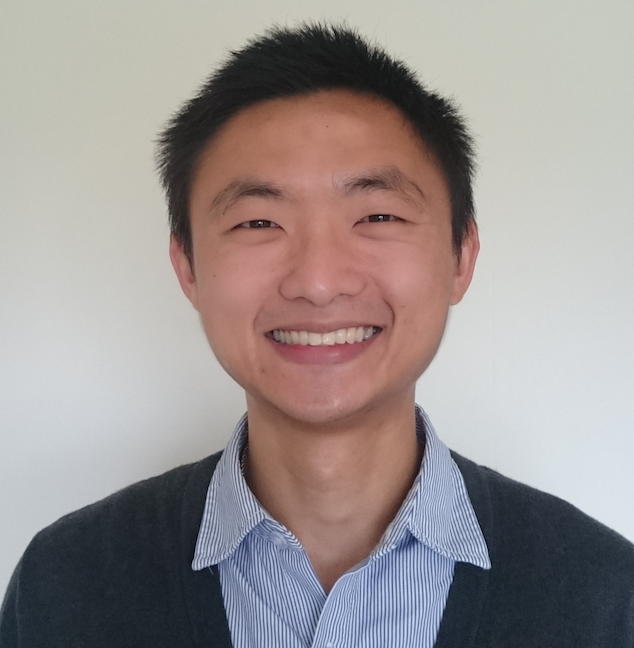
\includegraphics[width=\textwidth]{profile.png}}
%\begin{tabbing} % Enables tabbing
%\hspace{3cm} \= \hspace{4cm} \= \kill % Spacing within the block
%% {\bf Nationality} \> Taiwan \\ % Nationality 
%% {\bf Address } \> \\
%% Gersonsvej 75 st th\\ % Address line 1
%% 2900, Hellerup \\
%% Denmark\\\\ % Address line 2
%% {\bf Date of Birth} \> \\
%% 14$^{th}$ December 1987 \\\\ % Date of birth 
%% {\bf Contact } \> \\
%+45 50 12 28 50 \\ % Mobile phone
%spencer.tengz@gmail.com \\ % Email address
%https://www.linkedin.com/in/spencerimp/ \\ % LinkedIn
%\end{tabbing}
%\end{minipage}

\noindent\begin{minipage}[t]{0.8\textwidth}
	\vspace{0.5em}
	Versatile data scientist with multi-year hand-on experience building AI-powered applications such as music recommendation, medical image analysis, and chatbot. Goal-oriented, autonomous, and strong problem-solving engineer. Looking for a new journey to assist healthcare workers by using machine learning and software engineering technology. 
%%----------------------------------------------------------------------------------------
%%	SKILLS SECTION
%%----------------------------------------------------------------------------------------
\section{Skills}

Python, Machine Learning, Deep learning, Keras, TensorFlow, Scikit-learn, Pandas, Matplotlib \\
Django REST Framework, Git, Docker, Jenkins, Linux/Unix, Scrum \\
\end{minipage}\hspace{1mm}
\begin{minipage}[t]{0.2\textwidth}
\raisebox{\dimexpr-\height+\ht\strutbox}{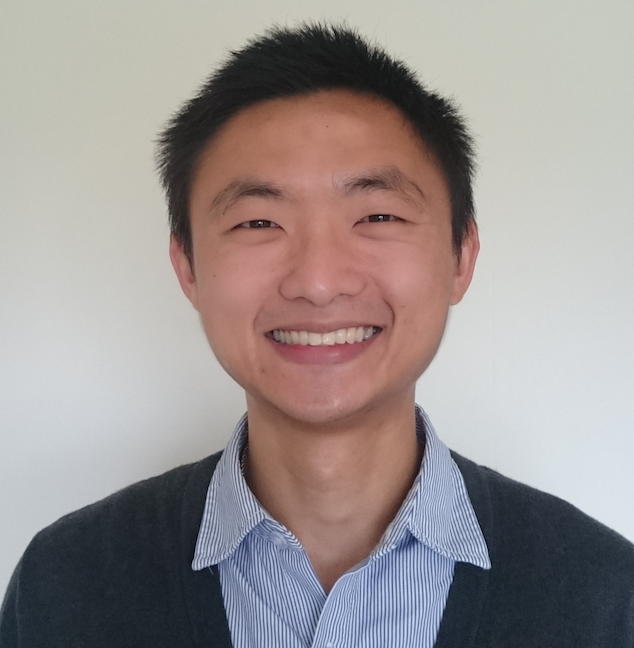
\includegraphics[height=\textwidth]{profile.png}}
spencer.tengz@gmail.com
linkedin.com/in/spencerimp/
+4550122850
\end{minipage}
%----------------------------------------------------------------------------------------
%	Experience
%----------------------------------------------------------------------------------------

\section{Experience}
\job
{Oct 2018 }{Present}
{\textbf{Data Scientist}}
{}
{Natural Language Processing, Nordea Bank, CPH, Denmark}
{
	Developed Innova, Nordea in-house chatbot using Natural Language Processing techniques.
    \begin{itemize}
    	\itemsep-0.2em
    	\item Automated machine learning retraining and deployment in production.
    	\item Developed REST APIs to perform banking actions on behave of customers, which is long-awaited.
    	\item Tech stack: TensorFlow, Django Rest, Celery, Java Spring Boot, Elastic Stack, etc.
    \end{itemize}
}
\job
{Aug 2017 }{Jun 2018}
{\textbf{Technical Co-founder}}
{}
{GUTXY, Frederiksberg, Denmark}
{
 	\begin{itemize}
		\itemsep-0.2em
		\item Developed a bioinformatics product that provides a report to improve customers' gut health.  
		\item InnoFounder incubator program in 2018 (acceptance rate: 13/102).
		\item Tech stack: Scikit-learn, Django Rest, Qiime2, Matplotlib, AWS EC2, S3, ElasticBeanstalk, etc.
	\end{itemize}

}
\job
{Mar 2017 }{Present}
{\textbf{Machine Learning Engineer Freelancer}}
{}
{Upwork}
{
	Top-rated freelancer specialized in deep learning and computer vision systems.
 	\begin{itemize}
		\itemsep-0.2em
		\item Design and implement production-grade REST APIs for object detection, image segmentation, etc.
		\item Tech stack: Keras, TensorFlow, OpenCV, Scikit-learn, Django Rest, Docker, AWS EC2, S3, etc.
	\end{itemize}
}
\job
{Feb 2016 }{Feb 2017}
{\textbf{Research Assistant}}
{}
{Biomediq, CPH, Denmark}
{
 	\begin{itemize}
		\itemsep-0.2em
		\item Developed deep neural network based MRI segmentation pipeline and achieved the state-of-the-art.
		\item Published a book chapter about deep learning for brain MRI segmentation and analysis.
	\end{itemize}

}

\job
{Aug 2011 }{Aug 2014}
{\textbf{Research Assistant}}
{}
{Music AI Lab, Academic Sinica, Taipei, Taiwan}
{
 	\begin{itemize}
		\itemsep-0.2em
		\item Developed context-aware music recommendation app from data collection to prototyping for HTC.
		\item Published papers in conference and journal about recommendation and user behavior analysis.
	\end{itemize}


}
%----------------------------------------------------------------------------------------
%	EDUCATION SECTION
%----------------------------------------------------------------------------------------
\section{Education}
\tabbedblock{
\bf{2014-2016} \> M.Sc. Computer Science - University of Copenhagen CPH, Denmark\\
\>\+Master Thesis: Automated brain MRI segmentation with deep neural networks. \\ 
}
% %------------------------------------------------
% \tabbedblock{
% \bf{2006-2010} \> B.Sc. Computer Science - \textbf{National Taiwan Ocean University,} \\\>\+Keelung, Taiwan
% }

% %----------------------------------------------------------------------------------------
% %	INTERESTS SECTION
% %----------------------------------------------------------------------------------------

% \section{Interests \& Learning}
% Tennis, Cycling, Danish (modul 3)

\end{document}